% LaTeX-Vorlage zur Erstellung von Abschlussarbeiten an der FH Aachen
% Author: Sven Hinz
\RequirePackage{scrlfile}
\ReplacePackage{scrpage2}{scrlayer-scrpage}

\documentclass[12pt,a4paper]{scrreprt}

% Paket für Umlaute:
\usepackage[utf8]{inputenc}       % Cross Platform
%\usepackage[ansinew]{inputenc}   % Windows
%\usepackage[latin1]{inputenc}    % Linux
%\usepackage[applemac]{inputenc}  % Mac

\usepackage[ngerman]{babel}       % Sprache: deutsch
\usepackage{hyperref}   %links in TOC
\hypersetup{colorlinks=true, linkcolor=blue}
\usepackage{comment}
\usepackage{amsmath}
\usepackage{amsfonts}
\usepackage{amssymb}
\usepackage{makeidx}
\usepackage{graphicx}
\usepackage{epstopdf}
\usepackage{kpfonts}
\usepackage[left=2cm,right=2cm,top=2.5cm,bottom=2.5cm]{geometry}

\author{Sven Hinz} % --> Eigenen Namen einfügen

\usepackage[plainheadsepline,headsepline]{scrpage2}
\usepackage{color}
\usepackage{setspace}
\usepackage[numbers,square]{natbib}
\usepackage{longtable}
\usepackage{listings}
\usepackage{rotating}
\usepackage{pdfpages}
\usepackage{caption}
\usepackage{subcaption}
\parindent 0pt
\usepackage{booktabs}
\usepackage[export]{adjustbox}


% Schriftart
\usepackage{helvet}
\renewcommand{\familydefault}{\sfdefault}
\setkomafont{chapter}{\sffamily \large}
\setkomafont{section}{\sffamily \normalsize}
\setkomafont{subsection}{\sffamily \normalsize}
\setkomafont{subsubsection}{\sffamily \normalsize}
\addtokomafont{caption}{\sffamily \small}
\usepackage{courier}

% Abstand zwischen Kopfzeile und Kapitelüberschrift
\renewcommand*{\chapterheadstartvskip}{\vspace*{-0.75\baselineskip}}

% Einstellungen der Kopf- und Fußzeile
\pagestyle{scrheadings}
\ihead[\sffamily \bfseries \upshape \headmark]{\sffamily \bfseries \upshape \headmark}
\chead[]{}
\ohead[]{}
\ifoot[]{}
\cfoot[]{}
\ofoot[\sffamily \pagemark]{\sffamily \pagemark}
\automark[]{chapter}
\renewcommand*{\chapterheadendvskip}{\vspace*{1\baselineskip}}

% Formeln
\usepackage{fleqn} % linksbündig
\setlength{\mathindent}{1.5cm} % Einrücktiefe

% Tabellen
\usepackage{multirow} % mehrzeiliger Text in einer Spalte
\renewcommand{\arraystretch}{2} % Zeilenabstand vergrößern
\setlength{\doublerulesep}{0.1mm} % Abstand der Doppellinien verkleinern
\usepackage{tabu}
\newcolumntype{C}{>{\centering\arraybackslash$}p{3cm}<{$}}

% Quellcode / Kommandozeileneingabe
\lstdefinestyle{BashInputStyle}{
  language=bash,
  basicstyle=\small\ttfamily,
  %numbers=left,
  %numberstyle=\tiny,
  %numbersep=3pt,
  frame=tb,
  columns=fullflexible,
  %backgroundcolor=\color{yellow!20},
  linewidth=0.9\linewidth,
  xleftmargin=0.1\linewidth
}

% Inhalt
\renewcaptionname{ngerman}{\contentsname}{Inhalt} % Umbenennung in Inhalt

% Quellenverzeichnis
\renewcaptionname{ngerman}{\bibname}{Quellenverzeichnis} % Umbenennung in Quellenverzeichnis

%\usepackage[
%  tocindentmanual,
%  tocflat,
%  tocbreaksstrict,
%  toctextentriesleft,
%]{tocbasic}

% Abkürzungsverzeichnis
%\usepackage[intoc]{nomencl}
%\let\abbrev\nomenclature
%\renewcommand{\nomname}{Abkürzungsverzeichnis}
%\setlength{\nomlabelwidth}{.25\hsize}
%\renewcommand{\nomlabel}[1]{#1 \dotfill}
%\setlength{\nomitemsep}{-\parsep}
%\makenomenclature

\usepackage[]{acronym}

\begin{document}
\setstretch{1.25}
\addtocontents{toc}{\linespread{1}}

% Einbinden der Textinhalte mit '\include{...}'
% Die Dateien mit den Textinhalten befinden sich im Ordner 'doc'

\begin{titlepage}
	%ab hier kleinere Raender, mehr bedruckbare Flaeche.

	\thispagestyle{empty}
	\newgeometry{ left=0cm, right=0cm, top=0.6cm, bottom=0cm, includefoot}

	% FH Logo
	\begin{flushright}
		\includegraphics[width=1.7cm]{./pic/FHAC.jpg}
	\end{flushright}

	\vspace{-2.5cm}

	% Kopfzeile mit Fachbereich ...
	\centering \bfseries \Large FH~Aachen \\
	\vspace{0.5cm}
	\normalsize Fachbereich\\
	Maschinenbau~und~Mechatronik \\
	Studiengang~Produktentwicklung

	\vspace{1cm}

	%\centering \bfseries Bachelorarbeit
	\centering \bfseries Masterarbeit

	\vspace{0.8cm}

	%Titel der Arbeit
	\centering \begin{minipage}[t]{17cm}
		\centering \bfseries \large Der~Titel~der~Arbeit\\ ist~zweizeilig
		\medskip
	\end{minipage}

	\vspace{1.5cm}

	%Name und Matrikelnummer
	%\vspace*{1cm}
	%\hspace*{6.8cm}
	\begin{minipage}[t]{9cm}
		\centering Vorname Nachname \\ Matr.-Nr.: 123456
	\end{minipage}

	\vspace{2.1cm}

	%Professor und Betreuer
	%\vspace*{4.7cm}
	%\hspace*{6.8cm}
	\centering \begin{minipage}[t]{9cm}
		\centering \begin{tabular}{ll}
			Referent: & Prof. Dr-Ing. ...\\
			Korreferent: & Prof. Dr.-Ing. ...\\
			%Externer Betreuer: & Dipl.-Wirt.-Ing\\
		\end{tabular}
	\end{minipage}

	\vspace{7cm}

	% Firmenlogo
	%\begin{flushleft}
	%\centering \hspace{-8cm}
	%\begin{minipage}[t]{5cm}
			%\includegraphics[width=5cm]{./pic/firmenlogo.jpg}
	%\end{minipage}
	%\end{flushleft}


	%Erstellungsdatum
	%\vspace{-4cm}
	%\begin{flushright}
	\centering %\hspace{8cm}
	\begin{minipage}[b]{5cm}
			\centering
			\today\\ %Datum\\
			%\vspace{1cm}
			%In Zusammenarbeit mit\\
			%Firma, Ort\\
			%\vspace{1cm}
			%vertraulich bis xx.xx.xx
	\end{minipage}
	%\end{flushright}

	%\today
	\restoregeometry
\end{titlepage}


\clearpage
\chapter*{Erklärung}\label{erklaerung}
\markboth{Erklärung}{Erklärung}
Ich versichere hiermit, dass ich die vorliegende Arbeit selbstständig verfasst und keine anderen als die im Literaturverzeichnis angegebenen Quellen benutzt habe.

\bigskip

Stellen, die wörtlich oder sinngemäß aus veröffentlichten oder noch nicht veröffentlichten Quellen entnommen sind, sind als solche kenntlich gemacht.

\bigskip

Die Zeichnungen oder Abbildungen in dieser Arbeit sind von mir selbst erstellt worden oder mit einem entsprechenden Quellennachweis versehen.

\bigskip

Diese Arbeit ist in gleicher oder ähnlicher Form noch bei keiner anderen Prüfungsbehörde eingereicht worden.

\vspace{1cm}
Aachen, \today %Monat Jahr

\vspace{7cm}
%\section*{Geheimhaltung}\label{geheimhaltung}

%{\large\textbf{Geheimhaltung}}\\


%Die vorliegende Arbeit unterliegt bis ... der Geheimhaltung. Sie darf vorher weder vollständig noch auszugsweise ohne schriftliche Zustimmung des Autors, des betreuendes Referenten bzw. der Firma ... vervielfältigt, veröffentlicht oder Dritten zugänglich gemacht werden.

%\clearpage
\chapter*{Danksagung}\label{danksagung}
\markboth{Danksagung}{Danksagung}
Danke.

% Inhaltsverzeichnis
\clearpage
\makeatletter
\renewcommand*{\@dotsep}{1} % Punktabstand einstellen
\makeatother
    {
        \hypersetup{linkcolor=black}
        \tableofcontents
    }
\tableofcontents

% Das erste Kapitel soll auf einer ungeraden Seite beginnen.
\cleardoublepage
\setstretch{1.25}

% Nicht benötigte Kapitel können auskommentiert werden
% Für zusätzliche Kapitel müssen weitere Dateien im Ordner 'doc' angelegt werden

\clearpage
\chapter{\textbf{Einleitung}}\label{chap:Einleitung}
\addtocontents{toc}{\vspace{0.8cm}}

% TODO Einleitung schreiben
Hier steht bald eine Einleitung


%\newpage
 % einleitung
\clearpage
\chapter{\textbf{Vorwissen}}\label{chap:Vorwissen}
\addtocontents{toc}{\vspace{0.8cm}}
Im Folgenden werden ein paar grundsätzliche Sachverhalte und Definitionen festgelegt und erläutert. Sie sollen das Verständnis der Algorithmen in Kapitel \ref{chap:Lokalisierung - Lösungsansätze} ermöglichen und fördern. 


\section{bestimmbare Positionen}\label{sec:bestimmbare Positionen}
\addtocontents{toc}{\vspace{0.8cm}}
Die Position eines sich auf dem Boden bewegenden mobilen Roboters, in Bild \ref{fig:1a_dd}  eines sog. Differential Drive Roboters, kann angegeben werden durch 
$P=\mathbf{\begin{psmallmatrix}
x & y & \psi
\end{psmallmatrix}}^\intercal$.
Hierbei bezieht sich $x$ auf die Position gepeilt auf die x-Achse, $y$ die Position gepeilt auf die y-Achse und $\psi$  den Winkel zwischen der Ausrichtung des Roboters und der x-Achse. Die Literatur bezeichnet die erhaltene Position im Fall eines bodengebundenen Roboters als eine 2D Position.\\
Zur Positionsbestimmung eines UAVs kommt im Falle einer 3D Positionsbestimmung eine weitere Achse hinzu, sodass die 3D Position angegeben werde kann durch
$P=\mathbf{\begin{psmallmatrix}
x & y & z & \psi
\end{psmallmatrix}}^\intercal$.
Die zusätzliche Variable $z$ bezeichnet hierbei die Position des Roboters gepeilt auf die z-Achse. (siehe Bild \ref{fig:1b_uav})\\
Eine weitere Darstellung der Position eines UAVs ist die 6D Position. Hierbei kommen zu der eben besprochenen 3D Position zwei Winkel hinzu, wodurch die 6D Position angegeben werden kann durch
$P=\mathbf{\begin{psmallmatrix}
x & y & z & \psi & \theta & \varphi
\end{psmallmatrix}}^\intercal$.
Dies folgt einer Konvention der Luft-und Raumfahrt, dem Schiffbau und dem Automobilbau \cite{website:cosmos-indirekt}, wonach die Reihenfolge der Eulerschen Winkel in Gier-, Nick-, und Rollwinkel (engl. \textit{yaw, pitch, roll}) festgelegt ist. (siehe Bild \ref{fig:1c_euwinkel}) Der Winkel $\psi$ beschreibt folglich den Gierwinkel, $\theta$ den Nickwinkel und $\varphi$ den Rollwinkel. % Koordinatensystemsbilder für Positionen
\mbox{}
\begin{figure}
  \begin{subfigure}[t]{.3\textwidth}
    \centering
    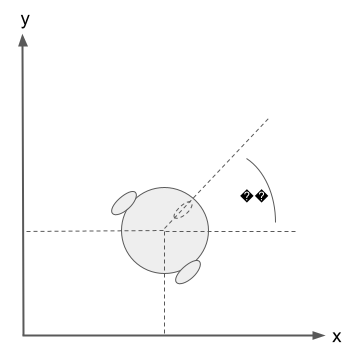
\includegraphics[width=.8\linewidth]{pic/vorwissen/1a_diffdrive.png}
    \caption{Position eines \textit{Differential Drive} Roboters}
    \label{fig:1a_dd}
  \end{subfigure}\hfill
  \begin{subfigure}[t]{.3\textwidth}
    \centering
    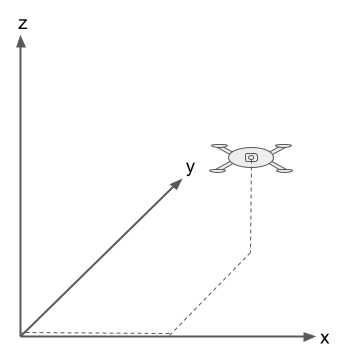
\includegraphics[width=.8\linewidth]{pic/vorwissen/1b_uav.png}
    \caption{Position eines UAV im dreidimensionalen Raum}
    \label{fig:1b_uav}
  \end{subfigure}\hfill
  \begin{subfigure}[t]{.3\textwidth}
    \centering
    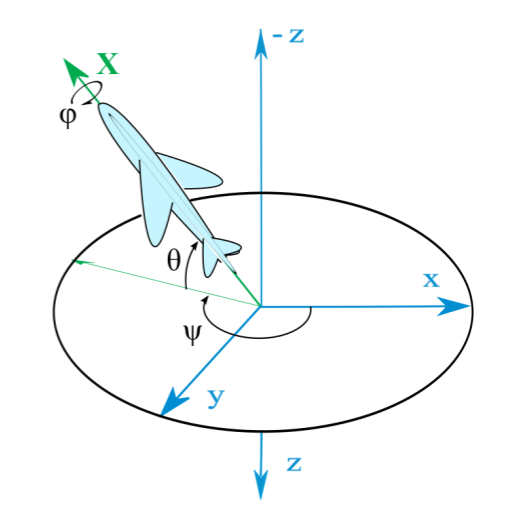
\includegraphics[width=.8\linewidth]{pic/vorwissen/1c_eulerwinkel.png}
    \caption{Konvention für Eulersche Winkel \cite{website:cosmos-indirekt-grafik}}
    \label{fig:1c_euwinkel}
  \end{subfigure}
  \label{fig:positionen}
\end{figure}
\mbox{}


\section{Kartenrepräsentation}\label{sec:Kartenrepräsentation}
\addtocontents{toc}{\vspace{0.8cm}}
Zur Positionsbestimmung in einer Karte ist die Auswahl der Kartenrepräsentation maßgebend. In der Kartendarstellung wird unterschieden zwischen einem topologischen- und einem metrischen Gerüst für eine Karte.\\
Bei einem topologischen Rahmen werden nur die Orte und dessen Beziehungen berücksichtigt, sodass die Karte ein Graph ist, bestehend aus Knoten, die die Orte repräsentieren und Bögen, die die Verbindungen der Orte darstellen. In einem metrischen Gerüst für eine Karte wird die räumlich-, Koordinatensystem-basierte Darstellung der Karte verwendet. Die Objekte innerhalb der Karte haben hierbei genaue Koordinaten.\\
Die in dieser Arbeit zumeist verwendeten Karten nutzen sogenannte \textit{Occupancy Grid Maps}. Hierbei wird ein Gitter mit definierter Masche auf die Karte gelegt. Befindet sich ein Objekt in der Karte, so wird jedes Gitterkästchen in dem sich das Objekt befindet als besetzt (engl. \textit{occupied}) gewertet und schwarz eingefärbt, wie in der Bilderreihe \ref{fig:occupanygridmap} dargestellt. So können die für eine Karte benötigten Datenmengen kontrolliert und eingegrenzt werden.\\
Im dreidimensionalen Raum können Occupancy Grid Maps ebenfalls eingesetzt werden. Der Raum kann dann nicht mehr nur mithilfe von zweidimensionalen Kästchen diskretisiert werden, sondern muss durch Würfel, sogenannte \textit{Voxel} eingeteilt und dargestellt werden.
\mbox{} % Biler Occupancy Grid Map 
\begin{figure}
  \begin{subfigure}[t]{.3\textwidth}
    \centering
    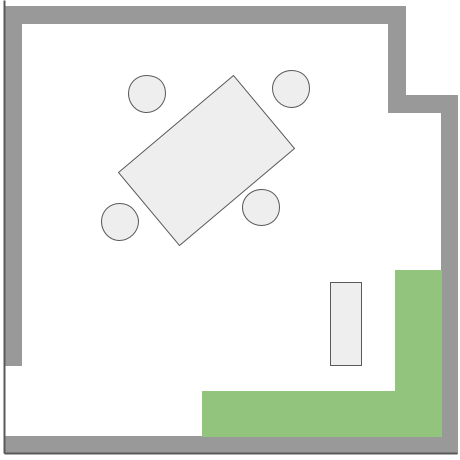
\includegraphics[width=.8\linewidth]{pic/vorwissen/2a_karte.png}
    \caption{Draufsicht eines Raumes}
  \end{subfigure}\hfill
  \begin{subfigure}[t]{.3\textwidth}
    \centering
    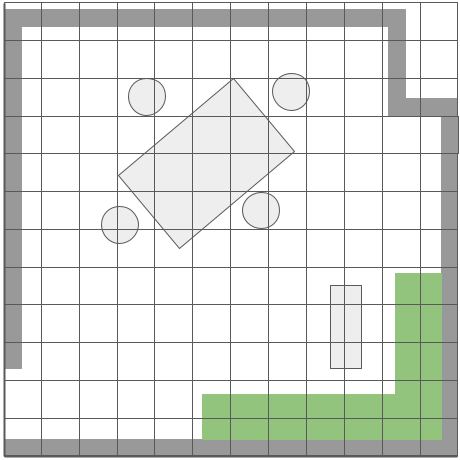
\includegraphics[width=.8\linewidth]{pic/vorwissen/2b_kartengitter.png}
    \caption{Einteilen des Raumes in gleichmäßig große Kästchen}
  \end{subfigure}\hfill
  \begin{subfigure}[t]{.3\textwidth}
    \centering
    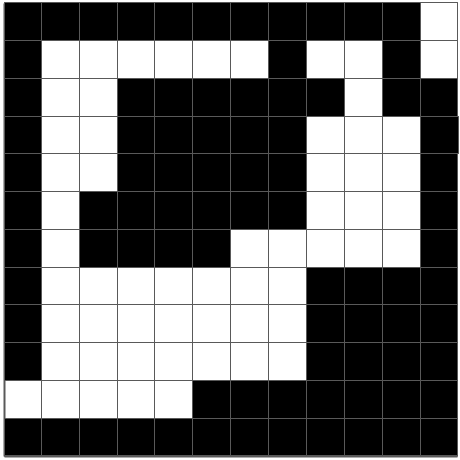
\includegraphics[width=.8\linewidth]{pic/vorwissen/2c_occupgridmap.png}
    \caption{Einfärben der besetzten Kästchen}
  \end{subfigure}
  \caption{Erstellen einer Occupancy Grid Map}
  \label{fig:occupanygridmap}
\end{figure}
\mbox{}


\section{Sensorik}\label{sec:Sensorik}
\addtocontents{toc}{\vspace{0.8cm}}
Die Sensorik eines mobilen Roboters kann unterteilt werden in interne- und externe Sensoren. Die internen Sensoren befinden sich innerhalb des Systems, und umfassen meistens Beschleunigungs-, Gyro- und gegebenenfalls Magnetometer Sensoren, welche für gewöhnlich in einer sogenannten \textit{Internal Measurement Unit} (IMU) zusammengefasst werden. Sie können genutzt werden, um ohne Wissen über die Außenwelt Aufschluss über die Position des Roboters über die Zeit zu geben. Dies wird auch als \textit{dead reckoning} bezeichnet, da sich die aktuelle Position nur aus der letzten errechneten Position errechnen lässt, welche bereits fehlerbehaftet sein kann. Da die Messung eines Sensors immer mit Messfehlern behaftet sein kann, wird auf diese Messung eine Art Toleranzbereich mit Wahrscheinlichkeitsverteilung angewendet, die oft einer Gaußschen Normalverteilung entspricht. (siehe Bild \ref{fig:3a_messunggauss}) Dadurch wird die Unsicherheit bzw. der Drift beim dead reckoning größer, je länger sich der Roboter ohne Berichtigung durch äußere Messungen fortbewegt. (siehen Bild \ref{fig:3b_growing_uncertainty})\\
Zu eben dieser Berichtigung durch äußere Messungen werden die externen Sensoren eingesetzt. Sie erfassen die den Roboter umgebende Welt durch beispielsweise Kameras, Ultraschallsensoren oder Laser-Range-Scanner. Auch die durch diese Sensoren gesendeten Messung können Messfehler enthalten, weswegen die Messungen wie die der internen Sensoren mit einem Toleranzbereich, dargestellt durch eine Wahrscheinlichkeitsverteilung, verrechnet werden.
\mbox{} % Bilder für Gaußsche Verteilung bei Messungen und Ungenauigkeiten bei Dead Reckoning
\begin{figure}
  \begin{subfigure}[t]{.5\textwidth}
    \centering
    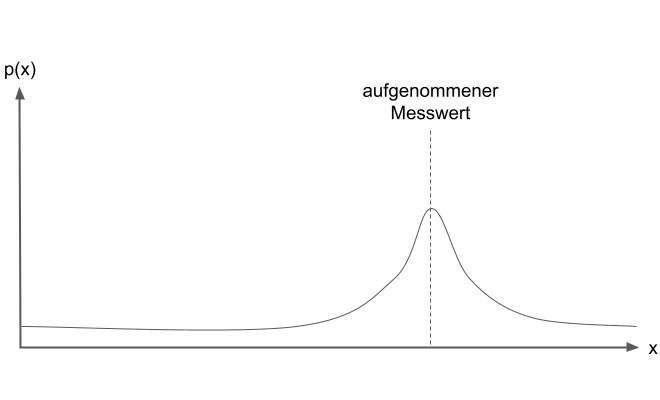
\includegraphics[width=.8\linewidth]{pic/vorwissen/3a_messunggauss.png}
    \caption{beschreibung}
    \label{fig:3a_messunggauss}
  \end{subfigure}\hfill
  \begin{subfigure}[t]{.5\textwidth}
    \centering
    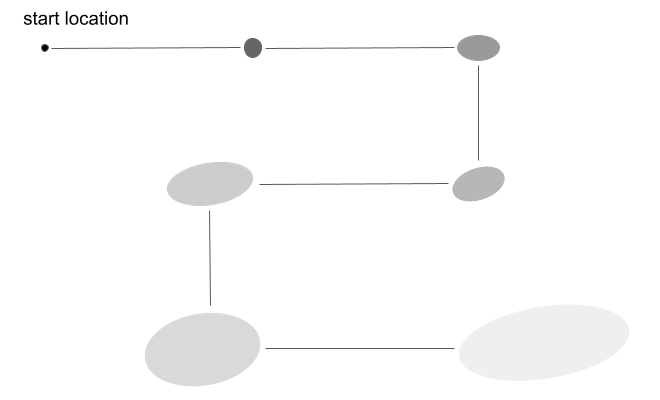
\includegraphics[width=.8\linewidth]{pic/vorwissen/3b_growinguncertainty.png}
    \caption{beschreibung}
    \label{fig:3b_growing_uncertainty}
  \end{subfigure}
\end{figure}
\mbox{}



\section{\textit{Motion-Model}}\label{sec:Motion-Model}
\addtocontents{toc}{\vspace{0.8cm}}
% TODO Motion-Model schreiben
hier wird bald was über das motion-model stehen

\section{\textit{Observation-Model}}\label{sec:Observation-Model}
\addtocontents{toc}{\vspace{0.8cm}}
% TODO Observation-Model
hier wird bald was über das observation-model stehen.



 % vorwissen
\clearpage
\chapter{\textbf{Lokalisierung - Lösungsansätze}}\label{chap:Lokalisierung - Lösungsansätze}
\addtocontents{toc}{\vspace{0.8cm}}
Das Themengebiet der Lokalisierung in der mobilen Robotik ist ein Grundstein für die Funktionalität dieser. Ohne Informationen über den genauen Standort könnte ein Räsenmäherroboter den Garten nicht schön halten, ein nach einem Paket greifenden UAV das Ziel nicht treffen oder eine Handvoll Fußball spielender Roboter den Ball nicht treffen. Dabei sind drei verschiedene Arten der Lokalisierung ausschlaggebend: Die \textit{Global Localization}, das \textit{Position Tracking} und die \textit{Kidnapping Recovery}. Die globale Lokalisierung beschreibt die Fähigkeit des Systems die korrekte erste Position in einer gegebenen Karte zu bestimmen. Das Position Tracking befasst sich mit der Aufgabe eine gefundene Position bei Bewegung des Systems beizubehalten, während die Kidnapping Recovery die Herausforderung beschreibt den Standort des mobilen Roboters nach einem Entführungsszenario wiederherzustellen. Ein Entführungsszenario meint hierbei das Bewegen des Systems, ohne dass die externen, Umgebung erfassenden Sensoren aktiv sind. In den folgenden Kapiteln werden ein paar Lösungsansätze und ausformulierte Algorithmen zur Lösung des Lokalisierungsproblems vorgestellt.

\section{Monte Carlo Localization}\label{sec:mcl}
\addtocontents{toc}{\vspace{0.8cm}}
Der von Daeller et al. \cite{Monte-Carlo-Localization} entwickelte \textit{Monte Carlo Localization} (MCL) Lokalisierungsalgorithmus verfolgt das Ziel einen mobilen Roboter in bekannter Umgebung zu orten. Der Algorithmus bekommt eine 2D Occupancy Grid Map, das Motion-Model und das Oberservation-Model des Systems zur Verfügung gestellt, generiert damit eine geschätzte 2D Position und ist in der Lage sowohl Position-Tracking, Globale Lokalisierung, als auch Kidnapping-Recovery zu absolvieren. \\
Es handelt sich hierbei um einen Partikelfilter, bei dem jedes Partikel eine mögliche Position des mobilen Systems ohne Toleranz darstellt. Die Einschätzung der Position $Bel(l)$ wird dargestellt durch ein \textit{N}-zahliges Set von gewichteten, zufälligen Partikeln oder \textit{Samples}.Ein Sample kann dargestellt werden durch $s=\langle\langle x,y,\psi \rangle,p\rangle$, wobei die $\langle x,y,\psi$ die Position, und $p$ das Gewicht beziehungsweise die Wahrscheinlichkeit dieser Position repräsentiert. Das Vorgehen ist eingeteilt in die Schritte \textbf{Robot Motion} und \textbf{Sensor readings}. Folglich wird der Algorithmus beginnend mit dem Schritt \textbf{Sensor readings} erläutert.\\
Im Beispiel \ref{fig:mcl} wird die eindimensionale Position eines mobiler Roboter berechnet, indem er auf einer Geraden an mehreren Türen entlang fährt. Ein außen montierter Sensor gibt an, ob er sich an einer Tür befindet. Zum Zeitpunkt der Intialisierung des Algorithmus wird das erste Set an Samples mit vollkommen willkürlichen Positionen, und dem Gewicht $p=N^{-1}$ generiert. Dann folgt der Schritt Sensor readings \ref{fig:s_mcl_sensor} wird das Observation-Model genutzt um die Umgebung wahrzunehmen, und von jedem individuellen Sample aus zu berechnen wie wahrscheinlich die erhaltene Messung an der Position \textit{l} des Samples ist. Die Gewichtungen $p$ der einzelnen Samples in dem Sample-Set werden dann entsprechend der Ergebnisse angepasst, sodass $\sum_{n=1}^{N} p_n =1$ gilt. Je wahrscheinlicher die reale Messung am Ort des Samples ist, desto höher ist dessen Gewichtung.\\
Es folgt der Schritt Robot Motion \ref{fig:s_mcl_motion}: Der Roboter bewegt sich, der Algorithmus generiert ein neues Set mit $N$ neuen Samples, die mithilfe des Motion-Models die neue Position nach der Bewegung annähern. Dafür werden per Zufallsverfahren Samples aus dem vorherigen Set entnommen gegebenenfalls vervielfacht und jedes Gewicht durch $N^{-1}$ ersetzt. Zusätzlich werden dem Set ein wenig neue Samples mit willkürlich generierten Positionen hinzugefügt. Das hilft dem System dabei sich im Falle eines Kidnapping-Szenarios neu zu lokalisieren. Anschließend macht der mobile Roboter wieder Gebrauch von seinem Observation-Model und führt den Schritt Sensor readings wieder aus. Das Partikel mit dem zuletzt höchsten Gewicht stellt die aktuelle Position des Roboters dar. Je mehr Iterationen durchgeführt werden, desto näher befinden sich die Partikel beieinander und desto genauer wird die angenäherte Position.
\mbox{}
\begin{figure}
  \begin{subfigure}[t]{.5\textwidth}
    \centering
    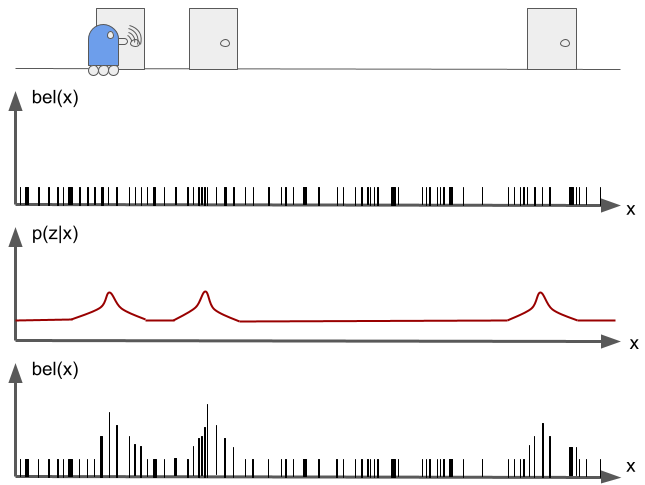
\includegraphics[width=.9\linewidth]{pic/loesungen/1a_mcl.png}
    \caption{Sensor readings}
    \label{fig:s_mcl_sensor}
  \end{subfigure}\hfill
  \begin{subfigure}[t]{.5\textwidth}
    \centering
    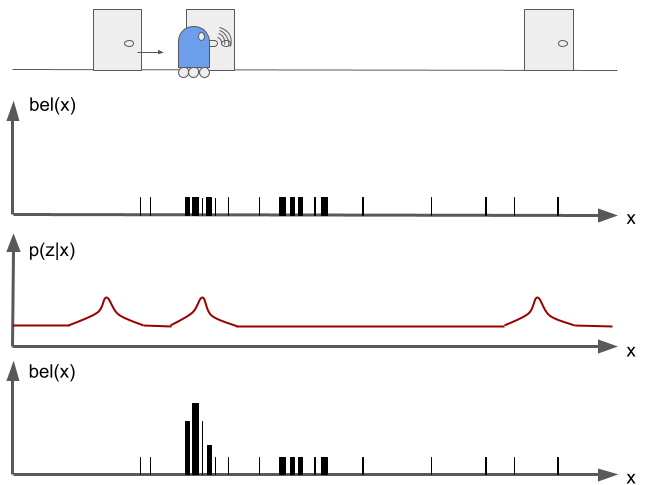
\includegraphics[width=.9\linewidth]{pic/loesungen/1b_mcl.png}
    \caption{Robot Motion}
    \label{fig:s_mcl_motion}
  \end{subfigure}
  \caption{Der MCL Algorithmus aufgeteilt in \textbf{Sensor readings} und \textbf{Robot Motion}}
  \label{fig:mcl}
\end{figure}
\mbox{}


\subsection{Adaptive Monte Carlo Localization}\label{subsec:amcl}
\addtocontents{toc}{\vspace{0.8cm}}
Der Adaptive Monte Carlo Localization (AMCL) Algorithmus ist eine leichte Abwandlung gegenüber des herkömmlichen MCL Algorithmus, der die Größe des Sample-Sets variiert. In MCL ist die Größe des Sample-Sets nach einmaliger Einstellung unveränderbar, dh. es werden für die Berechnung der Position in jeder Iteration die gleiche Menge an Partikeln benutzt. AMCL verfolgt das Ziel einer zumindest gleichwertigen, wenn nicht sogar besseren Positionsbestimmung wie MCL, will dabei aber ressourcenschonender sein. Das erreicht der Algorithmus, indem er die Anzahl der genutzten Partikel abhängig von der Unsicherheit über die errechnete Position dynamisch anpasst.\\
Das Position Tracking benötigt für eine genügend genaue Standortbestimmung wesentlich weniger zu berechnende Partikel, als die weitaus größere Herausforderung der globalen Lokalisierung oder der Kidnapping Recovery. Für die dynamische Festlegung der Größe der Sets wird die Abweichung zwischen dem \textit{belief} vor und nach der Messungen der externen Sensoren berechnet. Je größer hierbei die Überraschung der Sensordaten ist, desto größer wird das nächste Sample-Set gewählt. Der AMCL Algorithmus wird auch heutzutage, trotz seines Alters, in vielen Applikationen verwendet, da es schnell eine Position mit geringem Fehler berechnet.
% TODO Behauptungen hier belegen


\subsection{Monte Carlo Lokalisierung mit Surfel Grid Maps}\label{subsec:mcl_surfel}
\addtocontents{toc}{\vspace{0.8cm}}
\begin{wrapfigure}{R}{0.2\textwidth}
    \centering
    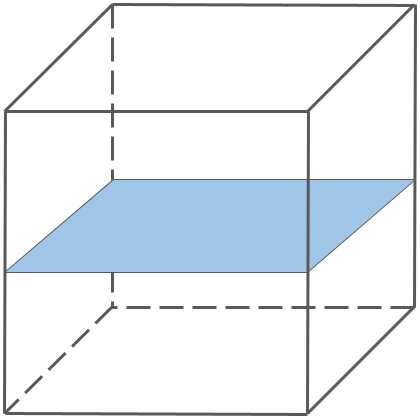
\includegraphics[width=0.18\textwidth]{pic/loesungen/12_surfel.png}
    \caption{Surface Element in a Voxel}
    \label{fig:surfel}
\end{wrapfigure}
Kläß et al. \cite{3DsurfelGridMaps} haben 2012 einen Algorithmus vorgestellt, dessen Ziel eine 2D Positionsbestimmung anhand einer 3D Voxel Grid Map ist. Die Lokalisierung wurde in der Veröffentlichung indoor durchgeführt und soll auch in dynamischen Szenarien, wenn sich beispielsweise bewegende Menschen in der Umgebung befinden, genau funktionieren können.\\
Die Besonderheit dieser Herangehensweise liegt in der Repräsentation der Umgebung. Die Umgebung wird durch eine vielzahl an Voxel (Würfel) modelliert, in denen sich jeweils ein \textit{Surface Element} oder kurz Surfel befindet (siehe bild). Befindet sich bei der Modellierung der Umgebung ein Objekt in einem Voxel, so wird ein Surfel entsprechend der Oberfläche des Objektes im Voxel generiert.\\
Die dahinter liegenden Berechnungen basieren auf MCL. Der Schritt Robot Motion bleibt bestehen, der der Sensor readings wird allerdings den neuen Techniken abgewandelt. Die Autoren schlagen für die verwendeten Sensor Models je nach Bedarf das \textit{Plane-to-Plane Model} oder das \textit{Line-to-Plane Model} vor. Ersteres stellt ein Oberservation-Model speziell für Sensorik, die 3D Scans in der 3D Surfel Grid Map durchführen soll, wie etwa LiDAR vor. Das Line-to-Plane Model hingegen zeigt eine mögliche Implementierung für Sensorik, die 2D Scans in der 3D Surfel Grid Map leisten soll. Aufgrund der fehlenden Dimension kann in letzterem Modell die Orientierung der Normale des Surfels nicht berücksichtigt werden.\\
Das System wurde vor allem in Hinblick auf die Navigation von bodengebundenen mobilen Robotern entwickelt. Das neuartige Surface Element soll dazu dienen die problematischen Diskretisierungseffekete von herkömmlichen 3D Voxel Grid Maps zu verringern (siehe Bild). Außerdem soll die Lokalisierung in dynamischen Szenarien erleichtert werden, indem der Algorithmus sich die 3D Map vollständig zu Nutze macht und sich dann auf Messungen über der Höhe des Menschen konzentriert um eine erfolgreiche Ortung durchzuführen.
% TODO Ergebnisse der Experimente einbringen
\mbox{}
\begin{figure}[ht]
  \begin{subfigure}[t]{.5\textwidth}
    \centering
    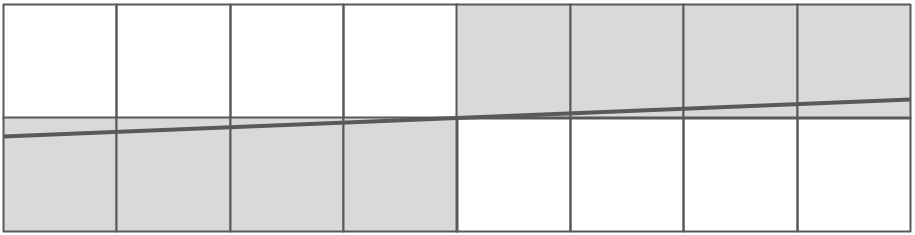
\includegraphics[width=.9\linewidth]{pic/loesungen/12a_steps.png}
    \caption{Generierung von Stufen}
    \label{fig:s_12steps}
  \end{subfigure}\hfill
  \begin{subfigure}[t]{.5\textwidth}
    \centering
    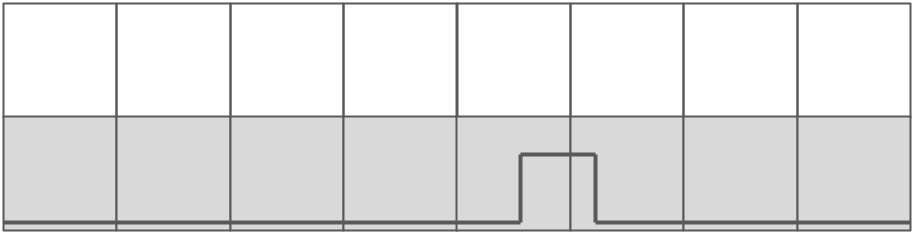
\includegraphics[width=.9\linewidth]{pic/loesungen/12b_bumps.png}
    \caption{}
    \label{fig:s_12bumps}
  \end{subfigure}
  \caption{typische Diskretisierungseffekte in Occupancy Voxel Maps \cite{3DsurfelGridMaps}}
  \label{fig:discretization_effects}
\end{figure}
\mbox{}

\newpage
\subsection{Dreidimensionale Indoor Lokalisierung}\label{subsec:3d_indoor}
\addtocontents{toc}{\vspace{0.8cm}}
\begin{wrapfigure}{R}{0.5\textwidth}
    \centering
    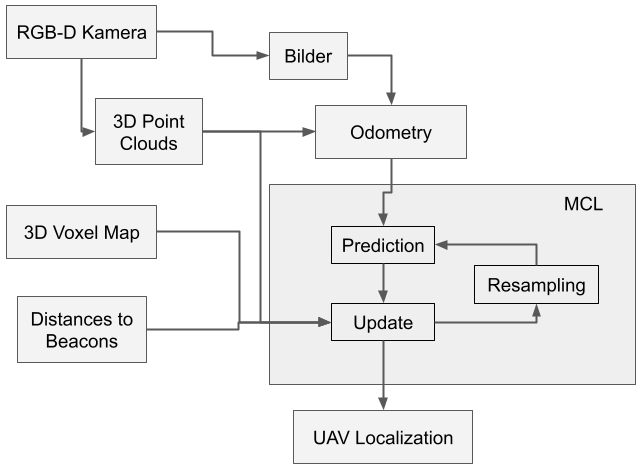
\includegraphics[width=0.48\textwidth]{pic/loesungen/13_system.png}
    \caption{Systemaufbau}
    \label{fig:13_system}
\end{wrapfigure}
Perez-Grau et al. \cite{dreidimensionale_indoor_lokalisierung} haben 2017 ein System zur dreidimensionalen Positionsbestimmung eines UAV in einem geschlossenen Raum vorgestellt. Der Ansporn zu dessen Entwurf liegt in der industriellen Nutzung von UAVs, wie beispielsweise dem Transportieren von Gegenständen.\\
Die Umgebung wird in Voxeln modelliert und es werden mehrere Sensoren benutzt um mithilfe des MCL Algorithmus eine 3D Position errechnen zu können (siehe Bild \ref{fig:13_system}). Eine RGB-D Kamera wird genutzt um sowohl RGB-Bilder, als auch Point Clouds erfassen zu können. Außerdem werden drei sogenannte \textit{ultra-wideband Beacons} (UWB Beacons) genutzt, um per Triangulation einen Standort des UAVs im Raum errechnen zu können. Die Odometry ist hierbei nicht nur von einer IMU abhängig, sondern nutzt ebenfalls die Bilder der Kamera, als auch dessen Point Clouds. So soll eine möglichst genau \textit{Prediction} (Vorhersage) im Robot Motion Schritt des MCL generiert werden, die dann durch ein Update (Sensor readings) berichtigt wird. Diese Berichtigung ist abhängig von den 3D Point Clouds der Kamera, der 3D Voxel Map und den Distanzen zu den drei, im Raum verteilten, UWB Beacons. Die daraus errechnete 3D Position beinhaltet nicht die Nick- und Rollwinkel. Diese werden direkt aus den Berechnungen der IMU entnommen.\\
Der Raum in dem das System getestet wurde ist mit Kameras ausgestattet worden, um den wahren Standort des UAVs, unabhängig vom entworfenen System, erhalten zu können. So konnte ein mehr als 500 Sekunden langer Testflug unternommen werden, bei dem der Fehler der Odometry und der Fehler des MCL genau bestimmt werden konnten (siehe Bild \ref{fig:13_testergebnisse}).
\begin{figure}[ht]
    \centering
    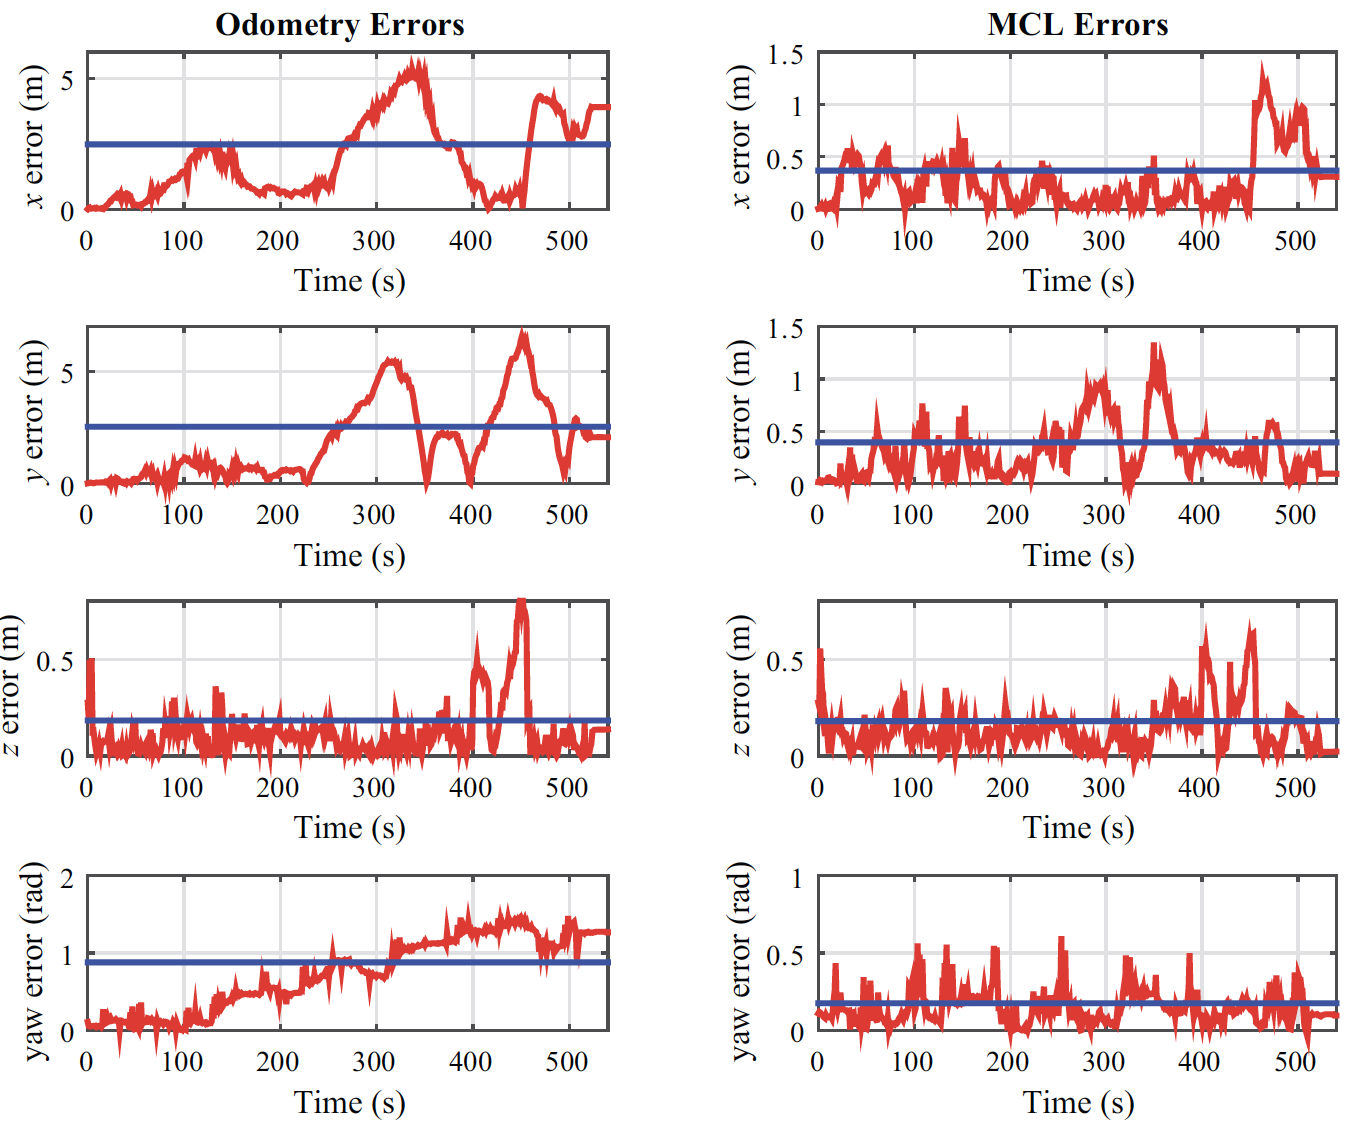
\includegraphics[width=0.9\textwidth]{pic/loesungen/13_testergebnisse.png}
    \caption{Testergebnisse der Autoren: links ist die Abweichung der Odometry, rechts die Abweichung nach Durchlauf des MCL angegeben \cite{dreidimensionale_indoor_lokalisierung}}
    \label{fig:13_testergebnisse}
\end{figure}


\section{Leader-Based Bat Algorithm}\label{sec:lbba}
\addtocontents{toc}{\vspace{0.8cm}}
Ähnlich wie die MCL, basiert der \textit{Leader-Based Bat Algorithm}(LBBA) ebenfalls auf Partikeln. Diese stellen in dem von Neto et al.\cite{LBBA} vorgeschlagenen Modell Fledermäuse dar, die ihre Inspiration in den \textit{Microbats} der realen Welt finden. Diese Fledermäuse fressen Insekten, und müssen ihre Umwelt und ihre Beute dazu präzise wahrnehmen können. Dazu fliegen sie an einem Ort \textit{x} mit einer Geschwindigkeit \textit{v} und nutzen die sogenannte Echolokation zur Wahrnehmung ihrer Umgebung. Dazu geben sie Ultraschallwellen von sich, nehmen die reflektierenden Wellen durch ihre Ohren wahr und bilden sich so ein Bild von ihrer Umwelt.\\
Yang et al.\cite{BA} implementierten und imitierten dieses Verhalten in dem \textit{Bat-Algorithm} (BA), dessen Aufgabenbereich in der globalen Optimierung liegt. Neto et al.\cite{LBBA} ergänzten diesen Algorithmus, mit dem Ziel ihn auf das Lokalisierungsproblem von mobilen Robotern anzupassen und darauf hin zu optimieren. Im Algorithmus werden $N$ viele Fledermäuse initialisiert, die eine zufällig zugeteilte Position $x$ und Geschwindigkeit $v$ haben. Außerdem wird die minimale- und maximale Frequenz,$F_{min}$ und $F_{max}$  (typischerweise [0,1]), die Lautstärke $A$ und die \textit{pulse emission rate} initialisiert. Der Ablauf des Algorithmus ist in Bild \ref{fig:lbba_code} dargestellt. Das Gewicht der Fledermäuse, bzw ihre \textit{fitness-function},, wird durch die Abweichung der am Ort der Fledermaus simulierten Sensor-Messung und der wahren Messung errechnet. Dies kann beispielsweise mithilfe des Observation-Models oder der Formel $f(x_i) = \frac{m_i -m}{m}$ erfolgen, wobei $m_i$ die simulierte Messung und m die wahre Messung darstellt.\\
\begin{figure}[ht]
    \centering
    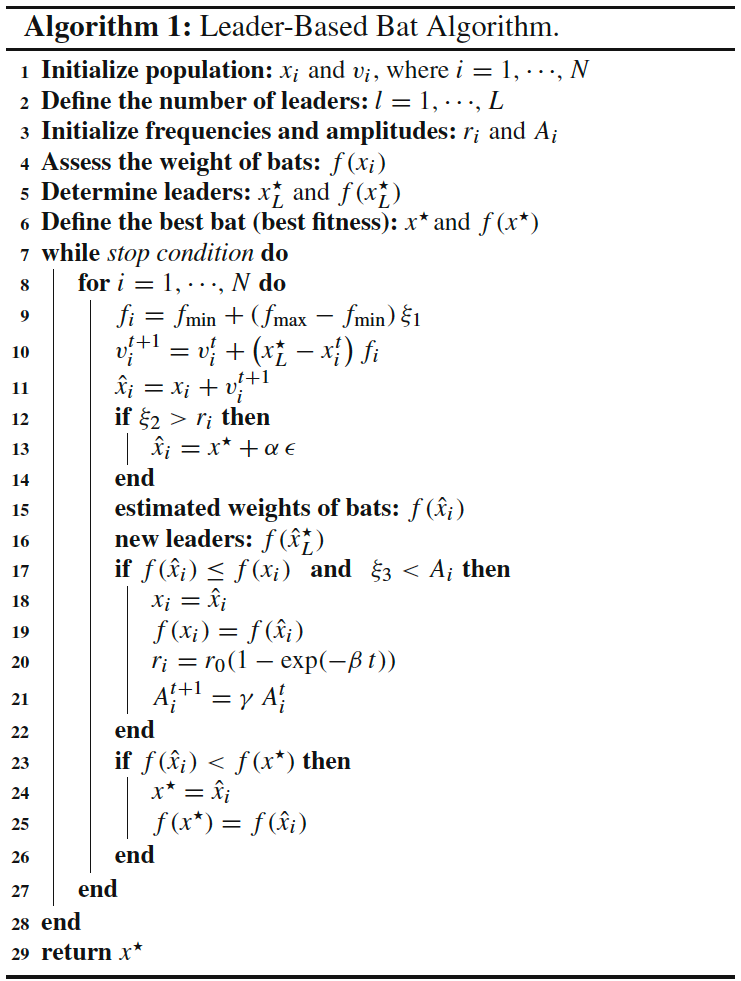
\includegraphics[width=0.5\textwidth]{pic/loesungen/20_lbba_algorithm.png}
    \caption{Der LBBA Code\cite{LBBA}. Die Variablen $\xi_{1-3}$ stellen zufällige Größen dar.}
    \label{fig:lbba_code}
\end{figure}
Der LBBA unterscheidet sich vom herkömmlichen BA in der Anzahl der besten Fledermäuse. Im BA wird bei jede Iteration genau eine Fledermaus zur besten Fledermaus in Hinsicht auf ihre fitness-Function gekürt. Dieser Alle anderen Fledermäuse bewegen sich in den darauf folgenden Iterationen auf diese Fledermaus zu, wobei eine Möglichkeit besteht, dass sie eine bessere fitness-Function als die ehemals beste Fledermaus haben, womit sie wiederum zur besten Fledermaus gekürt werden. Die Schleife wird so lange durchlaufen, bis ein Endkriterium erfüll wird. Im LBBA gibt es eine global beste Fledermaus, und eine benutzerdefinierte Anzahl an besten Fledermäusen. Alle Fledermäuse in einer bestimmten Nähe zur nächsten besten Fledermaus richten sich nach dieser aus und folgen dieser. Dies führt dazu, dass mehr Möglichkeiten der Lösung berücksichtigt werden, als im ursprünglichen BA.\\
Der LBBA ist im Kern ein offline-Algorithmus. Ihm genügt bereits eine Messung der externen Sensoren, um einen Standort errechnen zu können, was in der Aufgabe der globalen Lokalisierung von starkem Nutzen ist. Er kann allerdings auch online - also beispielsweise zum Position Tracking - eingesetzt werden. Die Autoren haben den LBBA unter anderem mit der AMCL und dem BA verglichen. Dabei haben sie experimentell festgestellt, dass LBBA mit nur wenigen Iterationen der \textit{while-Schleife} die präzisesten Ergebnisse liefert. Allerdings wird darauf hingedeutet, dass AMCL um ein vielfaches schneller ist sobald die globale Position einmal gefunden wurde.
 % Lokalisierung - Lösungsansätze

% beispiele von der Vorlage
%\include{./doc/101kap1} % Einleitung
%\include{./doc/102kap2}


% Nachspann
\nocite{waermeatlas} % Quelle wird nicht im Text erwähnt -> Quellenverzeichnis
\nocite{dubbel2005}
% Weitere quellen müssen in 'bib/quellen.bib' eingetragen werden
% !!! -> BibTex ausführen! Sonst tauchen die Quellen nicht im Verzeichnis auf.

% Quellenverzeichnis
\clearpage
\bibliographystyle{unsrtdin}
\bibliography{./bib/quellen}
\addcontentsline{toc}{chapter}{Quellenverzeichnis}
%\addtocontents{toc}{\vspace{0.8cm}}

% Abkürzungsverzeichnis
\clearpage
\markright{Abkürzungsverzeichnis}
\include{./doc/0abkuerzungsverzeichnis}
%\addtocontents{toc}{\vspace{0.8cm}}

% Abbildungsverzeichnis
\clearpage
\addcontentsline{toc}{chapter}{Abbildungsverzeichnis}
\listoffigures
%\addtocontents{toc}{\vspace{0.8cm}}

% Tabellenverzeichnis
\clearpage
\addcontentsline{toc}{chapter}{Tabellenverzeichnis}
\listoftables
\addtocontents{toc}{\vspace{0.8cm}}

% Anhaenge
\addcontentsline{toc}{chapter}{Anhang}
\appendix
%\input{./app/Dateiname}
\chapter{Datenblätter}
\begin{enumerate}
      \item Datenblatt 1
      \item Datenblatt 2
\end{enumerate}

% Anhänge im Ordner 'app' ablegen

%\includepdf[pages=1-4]{./app/Datenblatt1.pdf} % Datei mit 4 Seiten
%\includepdf[pages=1]{./app/Datenblatt2.pdf} % Datei mit einer Seite

\chapter{Konstruktionszeichnungen}
\begin{enumerate}
      \item Seitenansicht
      \item Draufsicht
\end{enumerate}
%\includepdf[pages=1]{./app/Seitenansicht.pdf}
%\includepdf[pages=1]{./app/Draufsicht.pdf}

\end{document}
